%Eddy
\documentclass[a0paper,portrait]{baposter}

\usepackage[font=small,labelfont=bf]{caption} % Required for specifying captions to tables and figures
\usepackage{booktabs} % Horizontal rules in tables
\usepackage{relsize} % Used for making text smaller in some places

\graphicspath{{figures/}} % Directory in which figures are stored

\definecolor{bordercol}{RGB}{40,40,40} % Border color of content boxes
\definecolor{headercol1}{RGB}{186,215,230} % Background color for the header in the content boxes (left side)
\definecolor{headercol2}{RGB}{80,80,80} % Background color for the header in the content boxes (right side)
\definecolor{headerfontcol}{RGB}{0,0,0} % Text color for the header text in the content boxes
\definecolor{boxcolor}{RGB}{186,215,230} % Background color for the content in the content boxes

\begin{document}

\background{ % Set the background to an image (background.pdf)
\begin{tikzpicture}[remember picture,overlay]
\draw (current page.north west)+(-2em,2em) node[anchor=north west]
{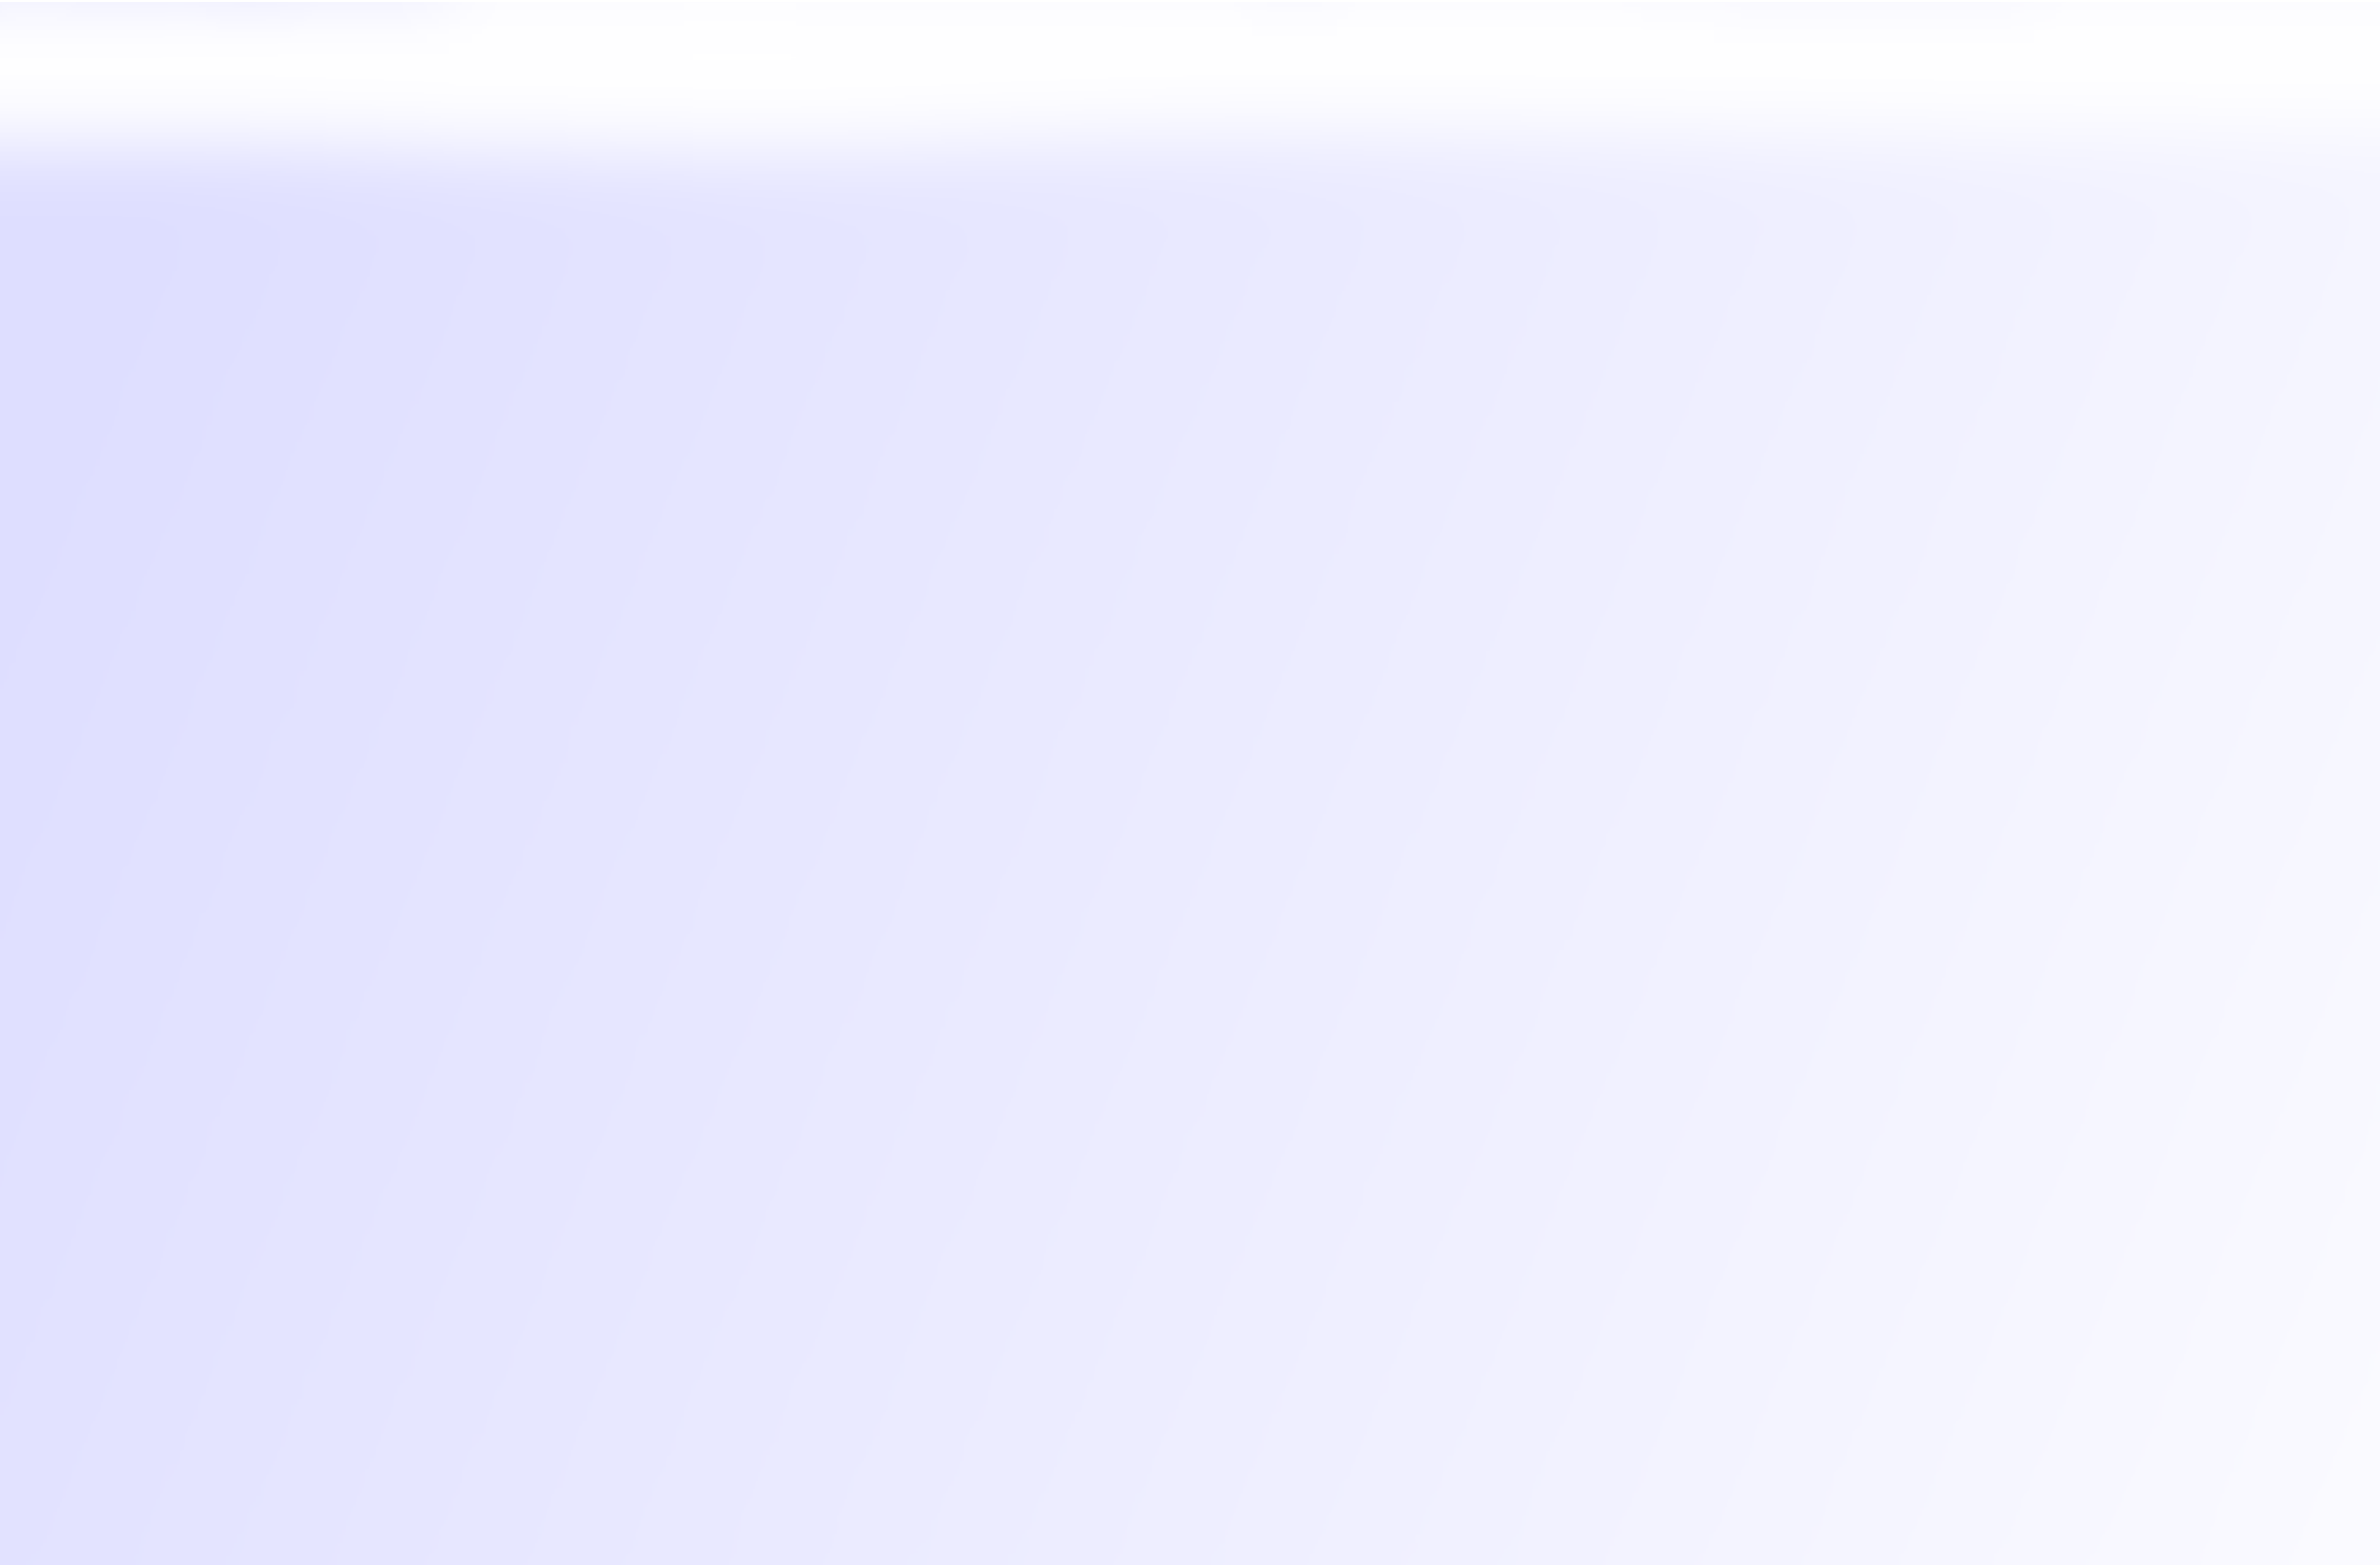
\includegraphics[height=1.1\textheight]{background}};
\end{tikzpicture}
}

\begin{poster}{
grid=false,
borderColor=bordercol, % Border color of content boxes
headerColorOne=headercol1, % Background color for the header in the content boxes (left side)
headerColorTwo=headercol2, % Background color for the header in the content boxes (right side)
headerFontColor=headerfontcol, % Text color for the header text in the content boxes
boxColorOne=boxcolor, % Background color for the content in the content boxes
headershape=roundedright, % Specify the rounded corner in the content box headers
headerfont=\Large\sf\bf, % Font modifiers for the text in the content box headers
textborder=rectangle,
background=user,
headerborder=open, % Change to closed for a line under the content box headers
boxshade=plain
}
{}
%----------------------------------------------------------------------------------------
%	TITLE AND AUTHOR NAME
%----------------------------------------------------------------------------------------
{\sf\bf Some Funny Yet \\ Relevant Title} % Poster title
{\vspace{1em} chriswangzanxu, 14102019, AjmastR, Anon, Or4nge, walnutt\\} % Author names
{
\includegraphics[scale=1.1]{the_logo}} % University/lab logo

%----------------------------------------------------------------------------------------
%	INTRODUCTION
%----------------------------------------------------------------------------------------

\headerbox{Introduction}{name=introduction,column=0,row=0}{
Introduction here
}

%----------------------------------------------------------------------------------------
%	AFH
%----------------------------------------------------------------------------------------
\headerbox{Adaptive Frequency Hopping}{name=AFH,column=0,below=introduction}{
\textbf{What Is Frequency Hopping?} \\
Adaptive Frequency Hopping (AFH) is a tehcnique where rather than using one single radiofrequency to transfer data, the frequency is constantly changing between a number of channels. This allows for both faster transfer speeds, and makes it harder for intruders to interfere with the signal. \\

\textbf{Why Is It Adaptive?} \\
The transmitting device is constantly monitoring the different channels to make an estimate of how good quality they are. For example, if one frequency is currently busy or being jammed, then it will simply use another channel.
}

%----------------------------------------------------------------------------------------
%	Another misc box
%----------------------------------------------------------------------------------------
\headerbox{Another General Box}{name=AGB,column=0,below=AFH}{
Box for another common feature (add more boxes as needed)
}

%----------------------------------------------------------------------------------------
%	CONCLUSION
%----------------------------------------------------------------------------------------

\headerbox{Conclusion}{name=conclusion,column=0,below=AGB}{
Conclusion here
}

%----------------------------------------------------------------------------------------
%	REFERENCES
%----------------------------------------------------------------------------------------

\headerbox{References}{name=references,column=0,below=conclusion}{

\smaller % Reduce the font size in this block
idk if we need this
\renewcommand{\section}[2]{\vskip 0.05em} % Get rid of the default "References" section title
\nocite{*} % Insert publications even if they are not cited in the poster

\bibliographystyle{unsrt}
\bibliography{sample} % Use sample.bib as the bibliography file
}

%----------------------------------------------------------------------------------------
%	ACKNOWLEDGEMENTS
%----------------------------------------------------------------------------------------

\headerbox{Acknowledgements}{name=acknowledgements,column=0,below=references, above=bottom}{
\smaller % Reduce the font size in this block
Rito
} 

%----------------------------------------------------------------------------------------
%	Wi-Fi
%----------------------------------------------------------------------------------------
\headerbox{Wi-Fi}{name=wifi,span=2,column=1,row=0}{ % To reduce this block to 1 column width, remove 'span=2'
Wi-Fi box here
}

%----------------------------------------------------------------------------------------
%	Optical Fibres
%----------------------------------------------------------------------------------------
\headerbox{Optical Fibres}{name=optical_fibre,span=2,column=1,below=wifi}{

\textbf {Introduction}
Optical fibres wires typically made from drawn silica glass, used to transmit information in the form of light pulses from lasers. It is made from a core of ultra-transparent material, surrounded by a transparent cladding with a lower refractive index. This allows for total internal reflection to occur within the core, confining light inside the fibre. Compared to copper wires, optical fibres offer greater information carrying capacity, immunity to electromagnetic disturbances, low attenuation loss and low production costs. Due to this, the advent of fibre optics greatly spurred on the development of the modern information era.\\

\textbf {Limitations of Optical Fibres} \\

\textbf{Residual Absorption}
Fundamental vibration frequencies of the particles that make up the glass absorbs light with matching frequencies.   

\textbf {Dispersion}
Dispersion is an optical phenomenon where light of different frequencies travel at different velocities through an optical medium: the higher the frequency, the slower it travels. In optical communications, data is coded in binary form and transmitted as pulses of light. As a single pulse from the laser carries more than one frequency of light, it is critical that the gap in time at the receiving end is not great than the time period ofthe wave group, otherwise the original data would be lost. This limits the maximum length of a single optical fibre, and requires the use of repeaters and/or amplifier to enable long distance communications, such as the trans-Atlantic cables. 

\textbf {Rayleigh Scattering}
The same unpreventable natural phenomena that makes the sky appear blue occurs inside the core of an optical fibre. An atom or molecule reradiates incident light in any direction except the incident direction. This effect is magnified at shorter wavelengths, and is increased by imperfections in the composition of the silica glass on a molecular level. 

}

%----------------------------------------------------------------------------------------
%	Bluetooth
%----------------------------------------------------------------------------------------
\headerbox{Bluetooth {
\includegraphics[scale=0.022]{bluetooth_logo}}}{name=bluetooth,span=2,column=1,below=optical_fibre}{
\textbf{History}
Bluetooth was developed by the Swedish telephone company Ericsson AB in
1990, and it first hit the commercial markets in 1999

\textbf{Master/Slave Topology}
Bluetooth follows a master/slave topology where there is a master device broadcasting data to a maximum of seven slave devices. This network of 8 devices is
known as a piconet. The master will always default to being the device which
initialised the connection, however master and slave roles can be exchanged
given that both devices agree upon this. 
{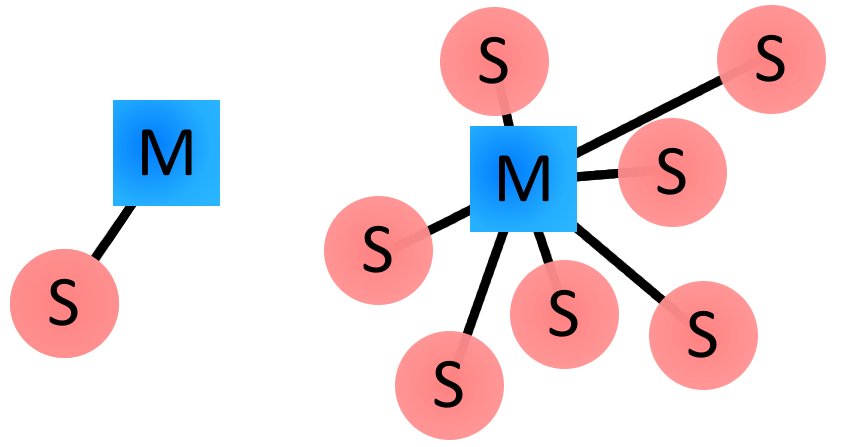
\includegraphics[scale=0.15]{master_slave_topology}} % University/lab logo

\textbf{AFH}
Bluetooth uses a technique known as AFH, which is explained on the left side of this poster.
}

%----------------------------------------------------------------------------------------
%	Li-Fi
%----------------------------------------------------------------------------------------
\headerbox{Li-Fi}{name=lifi,span=2,column=1,below=bluetooth}{
Li-Fi box here
}



%----------------------------------------------------------------------------------------
%	NFC
%----------------------------------------------------------------------------------------
\headerbox{NFC}{name=nfc,span=2,column=1,below=lifi}{
NFC box here
}

%----------------------------------------------------------------------------------------
%	Neutrinos
%----------------------------------------------------------------------------------------
\headerbox{Neutrino}{name=neutrino,span=2,column=1,below=nfc,above=bottom}{

\textbf{History}
Neutrino messaging is a hypothetical form of communication currently undergoing research. 
It was first experimentally verified to work in 2012 by researchers from the
University of Rochester and North Carolina State University.\\
\textbf{Advantages}
Unlike traditional forms of communication which rely on electromagnetic radiation, neutrinos are
affected only by the weak force and gravity, meaning they can pass messages through virtually
anything.
This can be utilised to transmit information across vast expanses in space, or for a more present-day application,
to send messages to nuclear submarines, as seawater can obstruct
electromagnetic radiation.\\
\textbf{Disadvantages}
The uninteractive nature of neutrinos causes them to be difficult to detect. Neutrinos also oscillate
between 3 flavours - electron, muon, and tau - this can be represented by a neutrino switching
between waves of different frequencies as it travels through space. This can be a
problem for certain detection methods.

}
\end{poster}

\end{document}